\documentclass[a4paper,11pt]{exam}
\usepackage[utf8]{inputenc}
\usepackage{enumerate}

%\usepackage{lipsum}

\date{\today}
\title{Introduction to Cloud Networking session 2: \\
\textit{Dockerizing} Distributed Applications}
\author{Simon Da Silva \and Mathias Lacaud}

%\usepackage{fancyhdr}
\usepackage{listings}
\usepackage{graphicx}

%\pagestyle{fancy}
%\fancyhf{}
\rhead{ENSEIRB-MATMECA}
\lhead{RE355 Introduction to Cloud Networking}


\lstset{language=sh,basicstyle=\ttfamily,columns=fullflexible}
\begin{document}
	
		
	
\maketitle


\section{Introduction}
\subsection{Installing docker compose}
Install Docker-Compose with:

\begin{lstlisting}[frame=single,language={sh}]  % Start your code-block

$ sudo curl -L "https://github.com/docker/compose/releases/download/1.22.0/
docker-compose-$(uname -s)-$(uname -m)" -o /usr/local/bin/docker-compose

$ sudo chmod +x /usr/local/bin/docker-compose

$ docker-compose --version
\end{lstlisting}

or alternatively, with \textit{pip}: 

\begin{lstlisting}[frame=single,language={sh}]  % Start your code-block

$ pip install docker-compose

$ docker-compose --version
\end{lstlisting}


\subsection{Basic Introduction to Docker Compose}

This is a quick description of \textit{docker compose}. If you don't know \textit{docker compose}, go through these explanations -- you will use them in the rest of the lab.
This introduction presents a simple web application that has two software components: a front-end and a server providing data.

\subsubsection*{Build images}
\begin{lstlisting}[frame=single,language={sh}]  % Start your code-block

# change directory and build image
$ cd intro/web
$ docker build -t re355/app .

# now the database
$ cd ../database
$ docker build -t re355/data
\end{lstlisting}

Now you can execute the application. The web server is listening on port 8080 and it depends on the database.

\subsubsection*{Executing the app (you should know this)}
\textit{Warning: You really have to use 'data' as the name. Do you know why it is necessary? Remember to kill and remove the containers when you are done playing.}

\begin{lstlisting}[frame=single,language={sh}]  % Start your code-block

$ docker run -d --rm --name data re355/data
$ docker run -d --rm -p 8080:8080 --link data re355/app 
      
\end{lstlisting}

Now you can go to the browser and enjoy this ``awesome'' application.

\subsubsection*{Using docker compose}
You have a \textit{docker-compose.yml} under the directory \textit{intro}:
\begin{lstlisting}[frame=single,language={sh}, tabsize=2, numbers=left]  
version: '2'
services:
	web:
		build:
			context: ./web
		image: re355/app:latest
		ports:
		- "8080:8080"
		links:
		- data

	data:
		container_name: data
		build:
			context: ./database
		image: re355/data       
\end{lstlisting}

In this docker compose file we are declaring two containers: \textit{web} (line 3) and \textit{data} (line 12).
They use images \textit{re351/web} and \textit{re351/data}.
In our case, this means using the Docker files inside directories \textit{./web} and \textit{./database}.
As you can see, the there is a port mapping (same as \textit{-p}), and the \textit{web} container is linked to \textit{data}.
Finally, in lines 5 and 15, we specify how to build the images if they don't exists. 

\subsection*{Deploying and stopping the composition}
\begin{lstlisting}[frame=single,language={sh}] % Start your code-block

# no need to speficy the file name. By default it uses docker-compose.yml.
$ docker-compose up

# play time ...

# then you can stop it using Ctrl+C or the command below
$ docker-compose down
\end{lstlisting}

You can use the flag \textit{-d} to launch the composition in detached mode. In such a case, using the \textit{down} subcommand is the only option to stop the composition. 
To see a description of each subcommand simply type:
\begin{lstlisting}[frame=single,language={sh}] % Start your code-block

# list of subcommands
$ docker-compose

# description of one subcommand
$ docker-compose up --help
\end{lstlisting}

\textit{Question}: what ip address is assigned to each container deployed? Are there differences in comparison to using \textit{docker} without docker-compose ?

Once you have finished this preliminary section, remove the images to save disk storage:
\begin{lstlisting}[frame=single,language={sh}] % Start your code-block

$ docker rm -f -v $(docker ps -a -q)
$ docker rmi re355/data re355/app
\end{lstlisting}

\subsection{Online documentation}
Additional information on docker compose can be found in the official online documentation~\footnote{https://docs.docker.com/compose/overview/}. Particularly,  in the compose file reference~\footnote{https://docs.docker.com/compose/compose-file/}.

\section{Dockerizing an application}

The idea of this TP is to deploy an application using Docker containers.
Currently, the application cannot be executed using docker. Your job is to ease the deployment of its components by using docker containers.
A high-level view of the applications is depicted in Figure~\ref{fig:architecture}.

\begin{figure}[!ht]
	\centering
	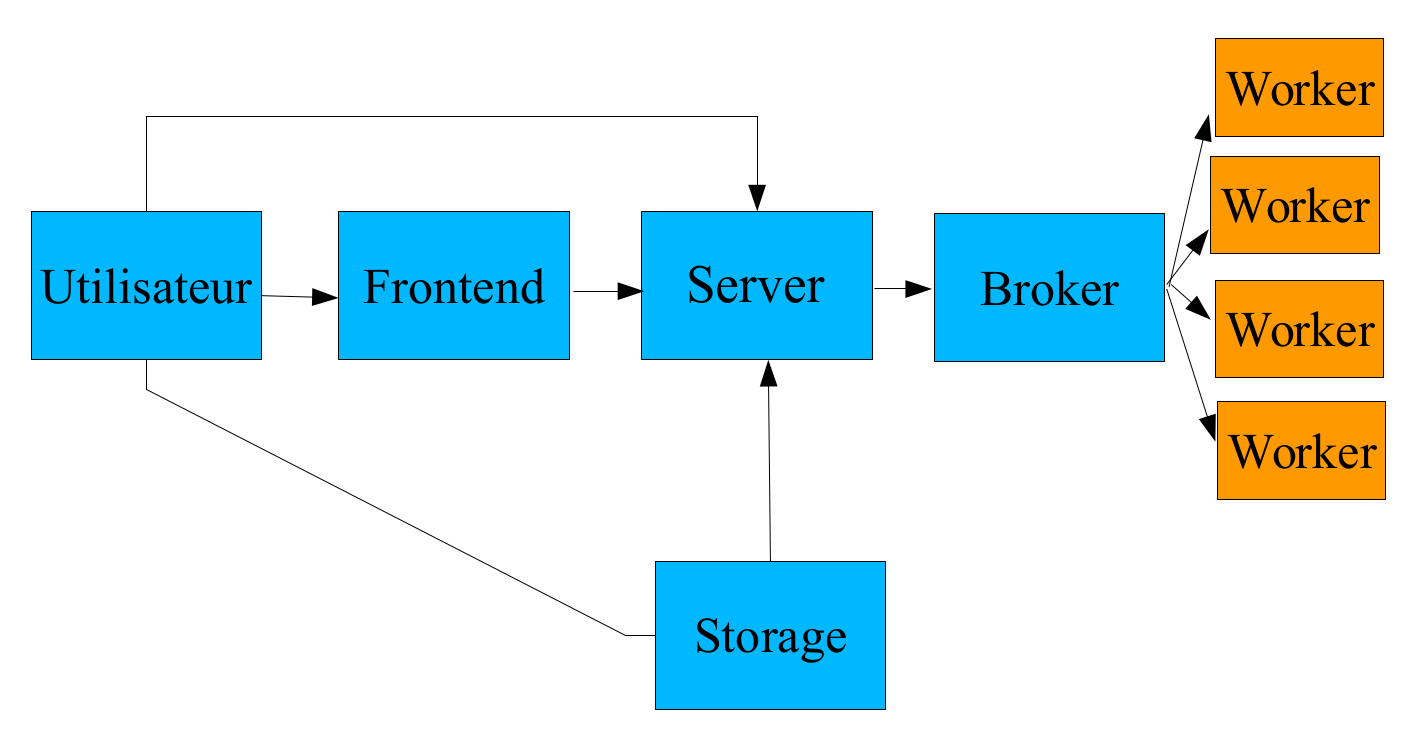
\includegraphics[width=0.8\textwidth]{fig/architecture.png}
	\label{fig:architecture}
\end{figure}

This application has five components that can be deployed in dockers containers.
Your task is to create a docker image for each component and a docker compose file to easily deploy the application.

Along the TP you will use the source code of the application. The code is in the \textbf{application} folder.

\subsection{Broker}

\begin{questions}
	\question The \textit{\textbf{Broker}} is simply a RabbitMQ server. Find and image in \textit{Docker Hub}~\footnote{https://hub.docker.com/explore/} and pull it.
	\begin{enumerate}[(a)]
		\item What is RabbitMQ?
		\item What is the standard port used in RabbitMQ?
		\item Create a \textit{compose} file and define a service ``broker'' based on the rabbitmq image.
	\end{enumerate}
\end{questions}
\subsection{Frontend}
\begin{questions}
	\question Define a Dockerfile for the \textit{\textbf{frontend}}.
	\begin{enumerate}[(a)]
		\item What base image can we use?
		\item What tools do you use to install the dependencies?
		\item Add the service to the \textit{compose} file.
	\end{enumerate}
Start your docker container. You should see in the logs: 
\begin{lstlisting}[frame=single,language={sh}]  % Start your code-block

ERROR
CORRECT USAGE: node index.js <server_ip>

Without the ip of the server, the frontend is useless by itself	
\end{lstlisting}
\begin{enumerate}[(d)]
		\item What is this error in the application? Fix it in the Dockerfile.
\end{enumerate}
	
	\textbf{Hints}:
	\begin{itemize}
		\item The application has been developped with NodeJS.
		\item You can use the \textit{alpine} tag of the base image to build a smaller frontend image.
		\item Remember that a \textit{Dockerfile} has: base image, copy source code, dependencies, entry point.
		\item The frontend is accessed through port 3000. You can access it using a browser.
		\item The dependencies must be installed by using \textit{npm install} 
		\item The server is executed using \textit{node index.js}.
		\item In this section and to encourage you to read the \textit{Hints}, the teachers won't answer your questions unless they begin with "Docker c'est génial, mais..."
	\end{itemize}
	\end{questions}
\subsection{Server}
	\begin{questions}

	\question Now it is time to dockerize the \textit{\textbf{server}}. Jump into the directory \textit{Server}. This component is far more complex than the \textit{\textbf{frontend}}. It is developped in Go (also called \textit{golang}). The component receives requests on port 8085.
	
	\begin{enumerate}[(a)] % (a)
		\item What base image can we use?
		\item Add the service to the \textit{compose} file.
		\item What are the modifications required in the previously defined services?
		\item How do you force the server to depend on the broker?
	\end{enumerate}
	Start your docker container. You should see in the logs something like: 
	\begin{lstlisting}[frame=single,language={sh}]  % Start your code-block
	
2018/10/30 16:21:09 dial tcp: lookup db on 192.168.1.142:53: no such host
exit status 1
		
	\end{lstlisting}
	\begin{enumerate}[(e)]
		\item Why the server fails during start-up?
	\end{enumerate}
	
	\textbf{Hints}:
	\begin{itemize}
		\item Find the ``right'' base image by searching in Docker Hub.
		\item Read the README.md of the Server
		\item \textit{"I do not understand why my server is not working. It should just connect to the database and... Wait ! Where is the database ?"} - a random student last year
	\end{itemize}
	\end{questions}


\subsection{Database}
	\begin{questions}
		\question The \textbf{server} needs a Mysql database to work. Let's dockerize the \textbf{storage}.
	
	\begin{enumerate}[(a)] % (a)
		\item What base image can we use?
		\item What is the default port of a mysql server?
		\item Add the service to the \textit{compose} file.
		\item What are the modifications required in the previously defined services?
	\end{enumerate}
		\textbf{Hints}:
	\begin{itemize}
		\item Find the ``right'' base image by searching in Docker Hub.

		\item The Server tries to connect to a database \textbf{re355}, with a username \textbf{re355} and a password \textbf{re355}.

		\item Remember that the environment variable MYSQL\_ROOT\_PASSWORD is mandatory.

		\item On the server side, use the \textbf{-d \textit{database\_addr}}

	\end{itemize}
	\end{questions}
	
\subsection{Waiting on startup}	
	\begin{questions}

	\question Sometimes, an application running within a container must wait until another container is ``ready'' (e.g., the web application of the introduction requires access to the database). However, when \textit{compose} deploys many services they are executed at the same time, without waiting. As a consequence, a container can fail because its dependencies are not ready. In the official documentation a solution is proposed~\footnote{https://docs.docker.com/compose/startup-order/}.
	
		\begin{enumerate}[(a)] % (a)
			\item What is wrong with the proposed solution?
			\item Why the application in the introduction doesn't fail? Take a look at the Dockefile in the folder \textit{introduction/web}
			\item How should you modify the \textit{\textbf{Server}}'s \textit{dockerfile} to fix this issue?
		\end{enumerate}
	\end{questions}
\subsection{Worker and full application}
	\begin{questions}
	
	\question Use file \textit{Worker/Dockerfile} to create the worker image. Afterwards, complete the \textit{composition} and deploy it. You can use the archive \textit{trailer.zip} in the frontend to answer the following questions:
	
	\begin{enumerate}[(a)] % (a)
		\item After uploading a video file, the results files are stored in which server? 
		\item Show your working application to your teacher. Who knows, he may give you a cookie... 
	\end{enumerate}
	
	\textbf{Hint:}
	\begin{itemize}
	\item The Worker need an environment variable \textbf{BROKER\_ADDR}. You can add it with \textit{-e BROKER\_ADDR=localhost:5672}
	\item You need to reload the webpage to update the list of available videos. 
	\end{itemize}
	\end{questions}


\subsection{Improving image size}	
	\begin{questions}

	\question By using \textit{docker images}, you can see the size of the images. The images are big because they are embedding all of the dependencies. However, as the Server image is written in Go, a langage that can be compiled, there is something we can do...
	
	\begin{enumerate}[(a)] % (a)
		\item In the Server folder, run an interactive container with a golang image. Bind a folder of the container with the current folder and indicate the command line you have used. (Hints: Take a look at the \textbf{-v} option of docker).
		\item Build the go project using the following line, and take a look at the folder. Can you see a new file?

		\begin{lstlisting}[frame=single,language={sh}]  % Start your code-block

			go build -tags netgo main.go

		\end{lstlisting}
		\item Change you Dockerfile to use \textit{alpine} as a base image. Copy the new file and run it. Build the new image. Take alook at its size. Conclude. 
	\end{enumerate}
\end{questions}
\section{Managing the resources of a cloud-based application}
\begin{questions}
	\question Let's assign some CPU quota to the web application we discuss in the introduction. Go to folder \textit{broken\_introduction} and deploy the application.
	
	\begin{enumerate}[(a)] % (a)
		\item What is the time needed to answer a request when no quota is used?
		\item Set a quota of 25\% of the CPU for the Web Container. What must be added to \textit{composition} file? 
		\item How long does it take to answer a request when the quota is 25\%?
	\end{enumerate}
	
	\question Suppose we have two clients accessing the application \textit{broken\_introduction}. We are offering them the same service but with a different quality. Modify the composition file to deploy a second \textit{web} container with a quota of 75\% of CPU.
	
	\begin{enumerate}[(a)] % (a)
	 	\item How long does it take to update the page? How are you testing this?
	\end{enumerate}
	
	\question We want to expose the previous application using the same URI for both clients (e.g., http://unique-addr:8888/) . This means that client 1 will connect to a service that has a CPU quota of 25\% and client 2 to a service with a quota of 75\%.
	 
	\begin{enumerate}[(a)] % (a)
		\item What tools should we use to achieve this?
		\item What should we modify in the \textit{composition} file?
		\item How can you test this new deployment?
	\end{enumerate}
	
\end{questions}

\section{Appendix}

At the end of this lab session, you will be rewarded by a beautiful red panda !
\begin{center}
	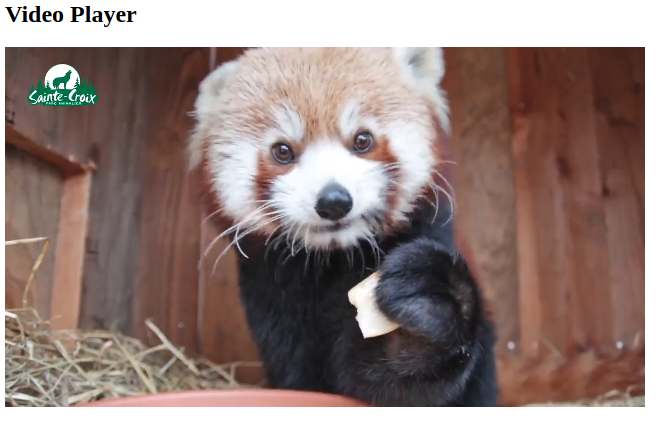
\includegraphics[width=12cm]{fig/redpanda.png}	
\end{center}


\end{document}
